\documentclass[
  captions=tableheading,
  bibliography=totoc, 
  titepage=firstiscover,
]{scrartcl}

\usepackage{blindtext} %neuer input

\usepackage{longtable} % Tabellen über mehrere Seiten

\usepackage[utf8]{inputenc} %neuer input

\usepackage{scrhack}

\usepackage[aux]{rerunfilecheck} %Warnung falls nochmal kompiliert werden muss

\usepackage{fontspec} %Fonteinstellungen

\recalctypearea{}

\usepackage[main=ngerman]{babel} %deutsche Spracheinstellung

\usepackage{ragged2e} %neuer input

\usepackage{amsmath, nccmath}

\usepackage{amssymb} %viele mathe Symbole

\usepackage{mathtools} %Erweiterungen für amsmath


\DeclarePairedDelimiter{\abs}{\lvert}{\rvert}
\DeclarePairedDelimiter{\norm}{\lVert}{\rVert}

\DeclarePairedDelimiter{\bra}{\langle}{\rvert}
\DeclarePairedDelimiter{\ket}{\lvert}{\rangle}

\DeclarePairedDelimiterX{\braket}[2]{\langle}{\rangle}{
#1 \delimsize| #2
}

\NewDocumentCommand \dif {m}
{
\mathinner{\symup{d} #1}
}


\usepackage[
  math-style=ISO,
  bold-style=ISO,
  sans-style=italic,
  nabla=upright,
  partial=upright,
  warnings-off={
    mathtools-colon,
    mathtools-overbracket,
  },
]{unicode-math}

\setmathfont{Latin Modern Math}
\setmathfont{XITS Math}[range={scr, bfscr}]
\setmathfont{XITS Math}[range={cal, bfcal}, StylisticSet=1]


\usepackage[
  locale=DE,
  separate-uncertainty=true,
  per-mode=reciprocal,
  output-decimal-marker={,},
]{siunitx}

\usepackage[autostyle]{csquotes} %richtige Anführungszeichen

\usepackage{xfrac}

\usepackage{float}

\floatplacement{figure}{htbp}

\floatplacement{table}{htbp}

\usepackage[ %floats innerhalb einer section halten
  section,   %floats innerhalb er section halten
  below,     %unterhalb der Section aber auf der selben Seite ist ok
]{placeins}

\usepackage[
  labelfont=bf,
  font=small,
  width=0.9\textwidth,
]{caption}

\usepackage{subcaption} %subfigure, subtable, subref

\usepackage{graphicx}

\usepackage{grffile}

\usepackage{booktabs}

\usepackage{microtype} %Verbesserungen am Schriftbild

\usepackage[
backend=biber,
]{biblatex}

\addbibresource{../lit.bib}

\usepackage[ %Hyperlinks im Dokument
  german,
  unicode,
  pdfusetitle,
  pdfcreator={},
  pdfproducer={},
]{hyperref}

\usepackage{bookmark}

\usepackage[shortcuts]{extdash}

%\usepackage{warpcol}

\usepackage{tikz}

\newcommand*\circled[1]{\tikz[baseline=(char.base)]{
            \node[shape=circle,draw,inner sep=2pt] (char) {#1};}}

\begin{document}
    \title{V903 Doppler-Sonographie}
    \author{  
    Tobias Rücker\\
    \texorpdfstring{\href{mailto:tobias.ruecker@tu-dortmund.de}{tobias.ruecker@tu-dortmund.de}
    \and}{,} 
    Paul Störbrock\\
    \texorpdfstring{\href{mailto:paul.stoerbrock@tu-dortmund.de}{paul.stoerbrock@tu-dortmund.de}}{}
    }
    \date{Durchführung: 07.07.2020, Abgabe: 17.07.2020\vspace{-4ex}}
\maketitle
\center{\Large Versuchsgruppe: \textbf{23}}
    
\newpage
\tableofcontents
\newpage

\setcounter{page}{1}

\section{Ziel}

    \flushleft{Die\;}\justifying Doppler-Sonographie hat viele Anwendungsmöglichkeiten in der Medizin. Sie kann beispielsweise dafür verwendet werden Blutgerinsel in Blutgefäßen zu orten
    oder um das Befinden eines Embryos zu überprüfen. Ziel dieses Versuches ist es die Strömungsgeschwindigkeit und das Strömungsprofil eines Rohres mithilfe der Doppler-Sonographie
    zu untersuchen. 

\section{Theorie}

    \flushleft{Die\;}\justifying Doppler-Sonographie nutzt den Doppler-Effekt aus um den Fluss innerhalb eines geschlossenen Systems bestimmen zu können. Der Doppler-Effekt 
    beschreibt die Streckung, bzw. Stauchung einer Wellenlänge im bewegten Bezugssystem. Bewegt sich die Quelle auf den Beobachter zu, wird die Wellenlänge gestaucht, also die
    Frequenz $\nu_0$ zu $\nu_{\text{gr}}$ vergrößert. Umgekehrt vergrößert sich die Wellenlänge sobald sich die Quelle von dem Beobachter wegbewegt, wodurch die Frequenz kleiner wird 
    $\nu_{\text{kl}}$. Daraus ergibt sich das folgende Verhältnis für die jeweils enstehende Frequenz: 
    \begin{align}
        \nu_{\text{kl/gr}} &= \frac{\nu_0}{1\mp \frac{v}{c}} \label{eq:1} \text{\cite{V903}}
    \end{align}
    \flushleft{Hierbei\;}\justifying ist $v$ die Geschwindigkeit, mit welcher sich der Beobachter auf die Quelle zu, bzw. von der Quelle wegbewegt und $c$ die Schallgeschwindigkeit.
    Im Falle, dass sich die Quelle in Ruhelage befindet und sich der Beobachter auf die Quelle zu, bzw. von der Quelle wegbewegt, lässt sich ein ähnliches 
    Verhältnis beobachten. Bewegt sich die Quelle auf den Beobachter zu, wird die Frequenz $\nu_0$ zu $\nu_h$ angehoben. Ebenso wird die Frequenz $\nu_0$ bei einer sich vom Beobachter 
    wegbewegenden Quelle auf $\nu_n$ gesenkt. Das daraus entstehende Verhältnis lautet wie folgt: 
    \begin{align}
        \nu_{\text{h/n}} &= \nu_0 \left( 1\pm \frac{v}{c} \right) \label{eq:2} \text{\cite{V903}}
    \end{align}
    \flushleft{Bei\;}\justifying der Doppler-Sonographie werden Ultraschallwellen an einem sich bewegenden Teilchen wie einem Blutkörperchen reflektiert. Die Bewegung des Blutkörperchens
    verursacht eine Frequenzverschiebung der Schallwelle, welche mit dem folgenden Aufbau zu messen ist.

\begin{figure}[H]
    \centering
    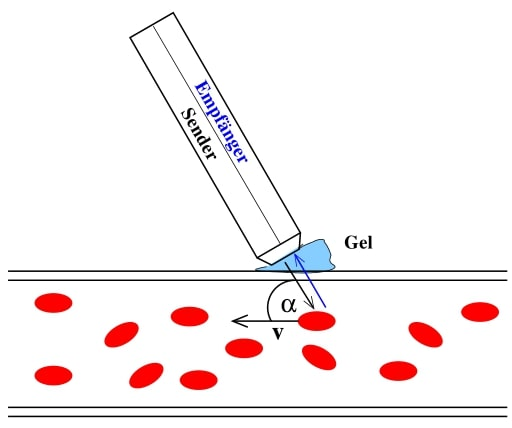
\includegraphics[width=0.5\linewidth]{images/Schema.jpg}
    \caption{In dieser schematischen Darstellung der Doppler-Sonographie \cite{V903} ist eine Sonde dagestellt. Diese beinhaltet einen Sender und einen Empfänger von Ultraschallwellen.
    Die Wellen fallen in einen Fluss von Teilchen (hier der Doppler-Flüssigkeit) ein und werden dort reflektiert. Der Winkel zwischen Wellennormalen und Geschwindigkeitsvektor des Teilchen ist $\alpha$
    oder $\beta$. Es wird bei den Winkeln zwischen einfallender und ausfallender Welle unterschieden, die in diesem Aufbau jedoch einen identischen Winkel besitzen. Das Gel sorgt dafür,
    dass die Schallwellen nicht von der Luft absorbiert werden.}
    \label{fig:1}
\end{figure}

    \flushleft{In\;}\justifying diesem Aufbau sind die Winkel $\alpha$ und $\beta$ zwischen Geschwindigkeitsvektor $v$ und den Wellennormalen der einfallenden und reflektierten Welle identisch. Die 
    entstehende Frequenzverschiebung $\Delta\nu$ lautet demnach wie folgt:
    \begin{align}
        \Delta\nu &= 2 \nu_0 \frac{v}{c} \cos \alpha \label{eq:3} \text{\cite{V903}}
    \end{align} 
    \flushleft{Die\;}\justifying Ultraschallwellen werden mithilfe des piezo-elektrischen Effekts gewonnen. Der piezo-elektrische Effekt beschreibt die Eigenschaft eines Piezokristalls,
    der in ein elektrisches Wechselfeld gehalten wird. Zeigt eine Polarachse des Kristalls in Richtung des E-Felds beginnt der Kristall zu schwingen. Diese Schwingung regen den Kristall an
    Ultraschallwellen abzustrahlen.
    Neben der Erzeugung von Ultraschallwellen kann ein Piezokristall auch als Empfänger verwendet werden, da Ultraschallwellen den Kristall ebenfalls zum schwingen bringen.\\
    Neben der Sonde wird noch ein Doppler-Prisma verwendet. Eine schematische Darstellung ist in der folgende Abbildung zu finden:

\begin{figure}[H]
    \centering
    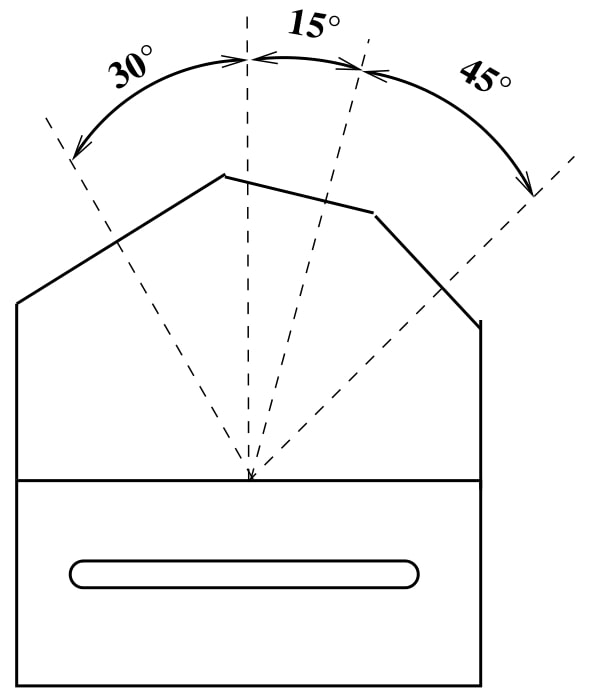
\includegraphics[width=0.35\linewidth]{images/Winkel.jpg}
    \caption{Diese Abbildung stellt das Doppler-Prisma dar \cite{V903}. Es erlaubt der Sonde drei Aufsetzmöglichkeiten, die jeweils einen festen Winkel zum darunterliegenden Rohr besitzen. Das
    Prisma ist so konstruiert, dass die Strecke zwischen Sonde und Rohr bei jedem Winkel gleich bleibt. Die hier abgebildeten Winkel sind \SI{15}{\degree}, \SI{30}{\degree} und \SI{45}{\degree}.}
    \label{fig:2}
\end{figure}

    \flushleft{Da\;}\justifying mit dem Doppler-Prisma ein weiterer Brechungswinkel eingeführt wird und die Sonde an drei Winkeln fixiert wird, ergibt sich aus dem Brechungsgesetz
    für den Winkel $\alpha$: 
    \begin{align}
        \alpha &= \text{\SI{90}{\degree}} - \arcsin\left( \sin(\theta) \frac{c_L}{c_P} \right) \label{eq:4} \text{\cite{V903}}
    \end{align}
    \flushleft{Hier\;}\justifying beschreibt der Winkel $\theta$ einen der drei fixierten Winkel \SI{15}{\degree}, \SI{30}{\degree}, oder \SI{45}{\degree}. $c_L$ ist die Schallgeschwindigkeit
    in der Doppler-Flüssigkeit und $c_P$ ist die Schallgeschwindigkeit des Prismenmaterials.

\newpage
\section{Vesuchsaufbau und Durchführung}

    \flushleft{Für\;}\justifying den Versuch wird folgender Versuchsaufbau verwendet:

\begin{figure}[H]
    \centering
    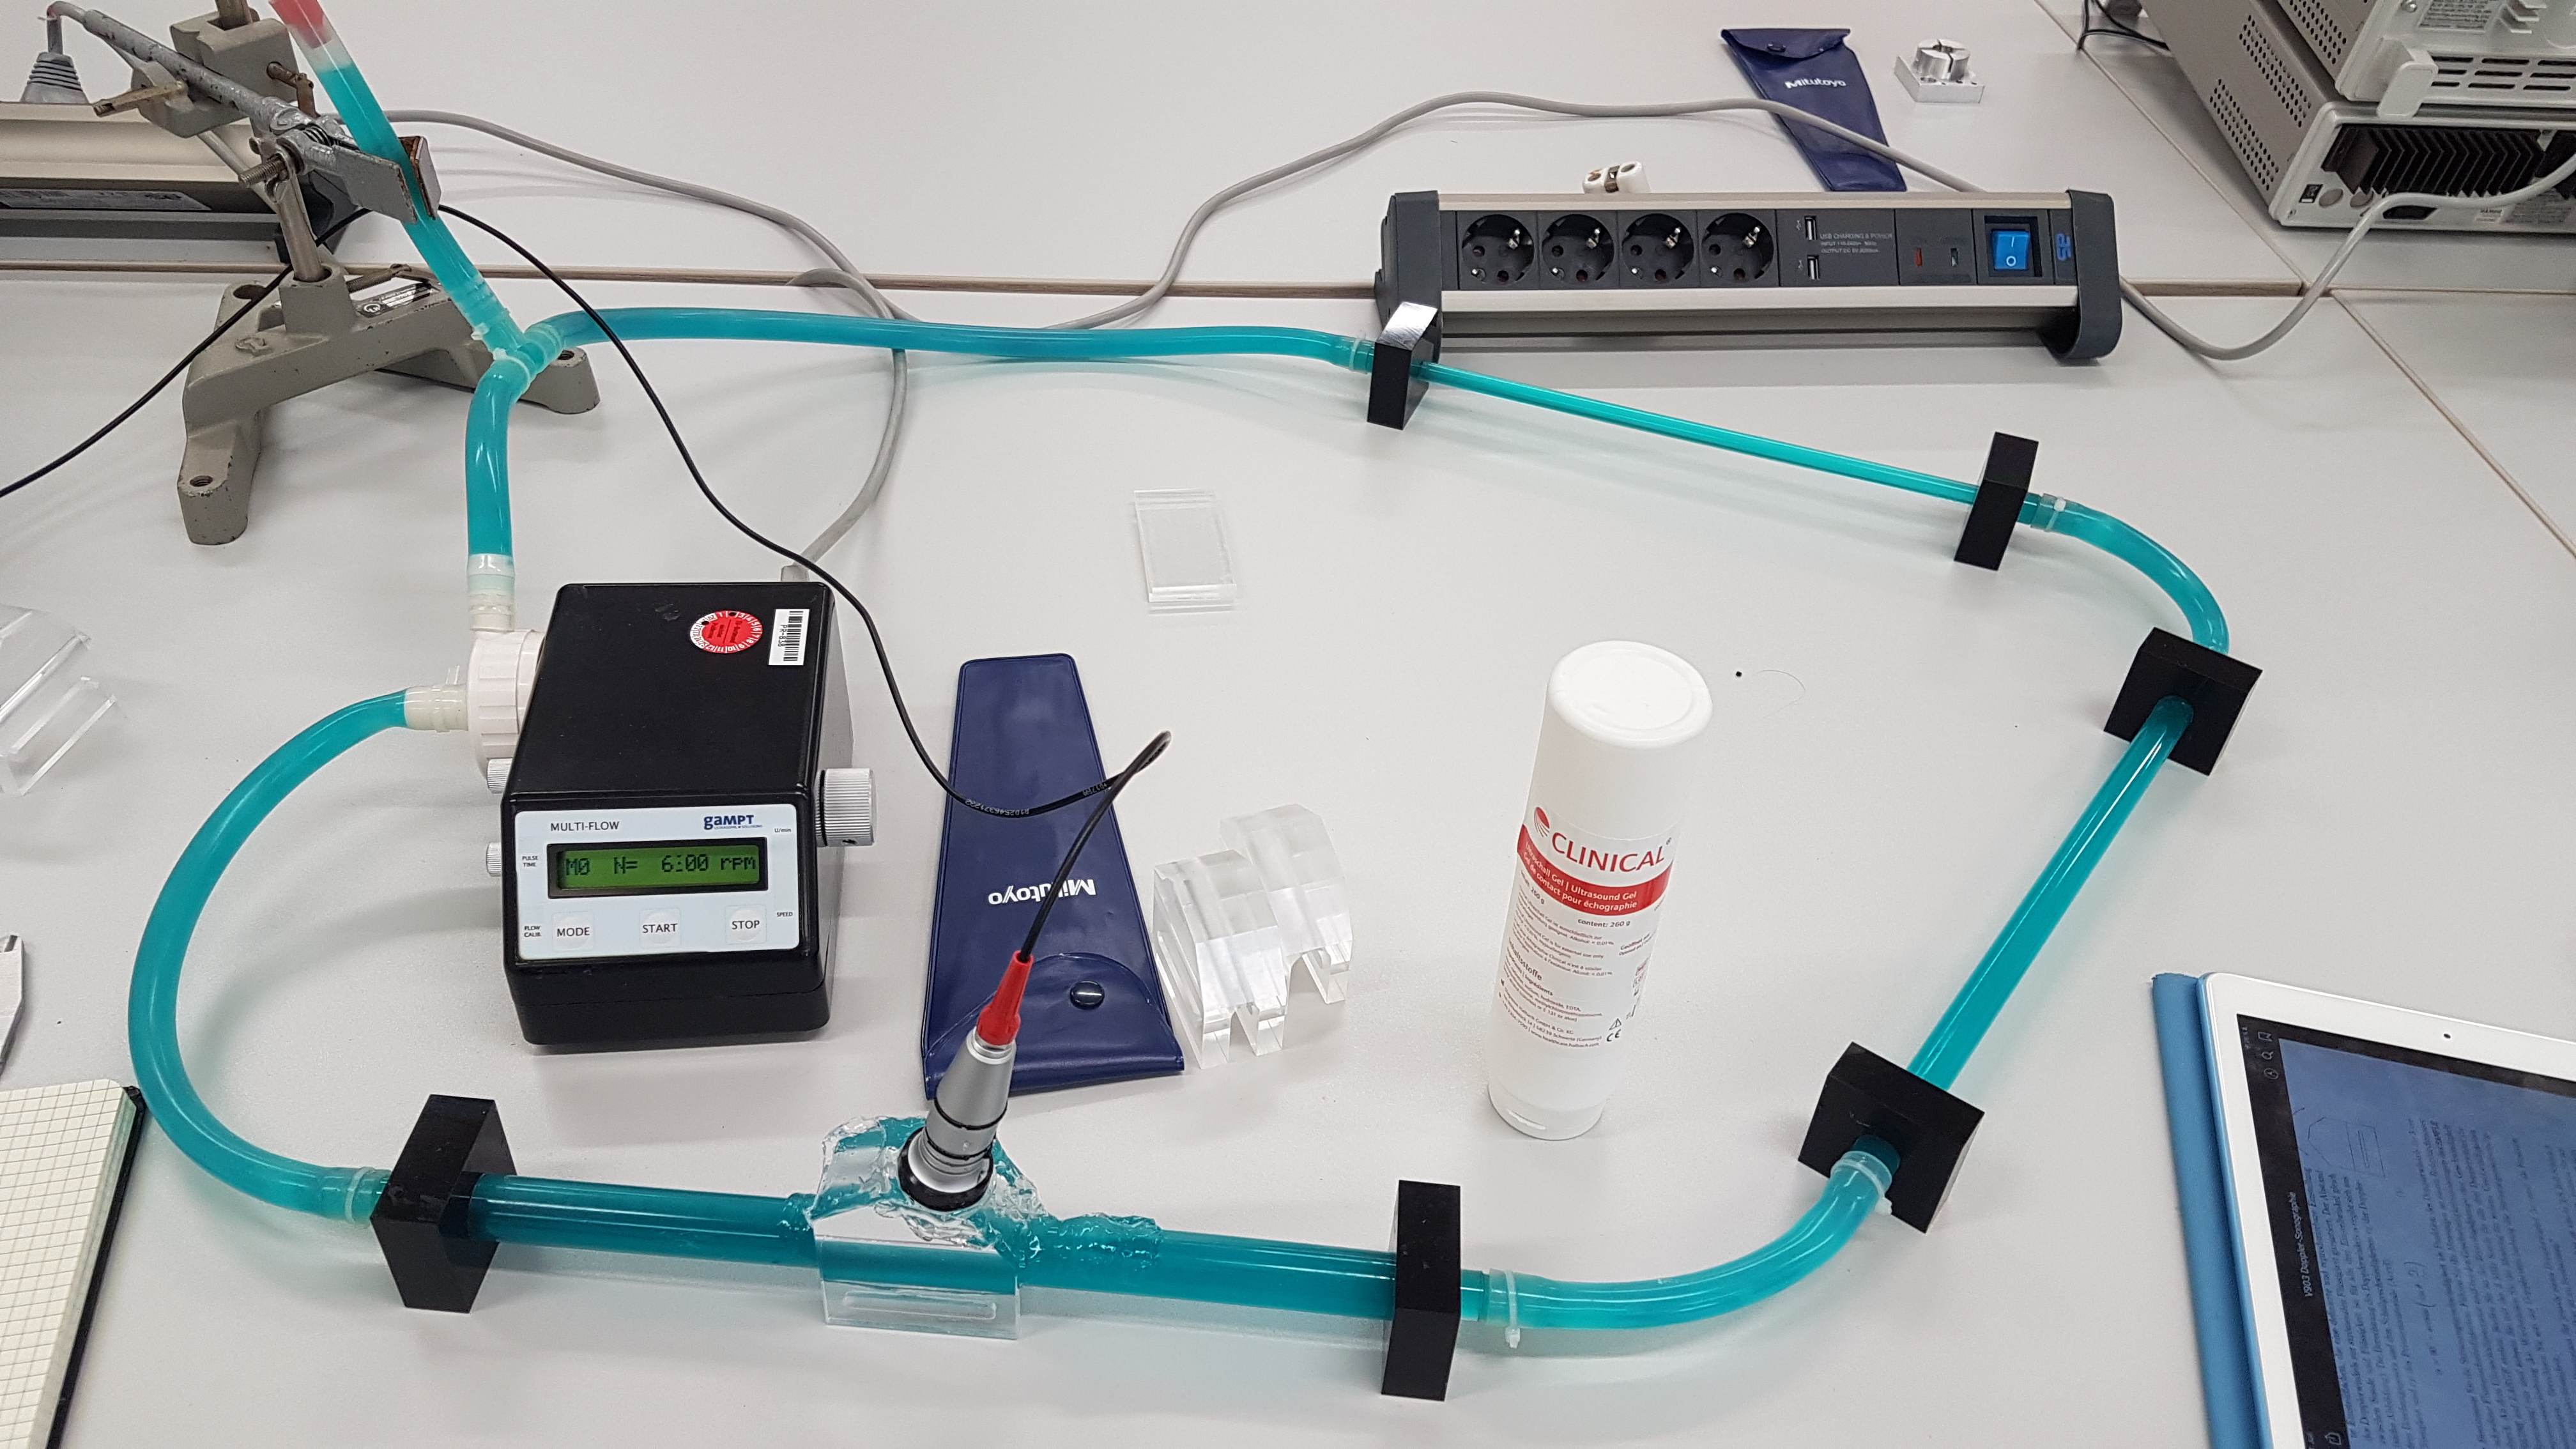
\includegraphics[width=0.75\linewidth]{images/Schlauch.jpg}
    \caption{In dieser Abbildung ist der Aufbau des Versuches zu erkennen. Der Versuch besteht aus einem Schlauch, der in vier Teile zerlegt werden kann. Ganz links befindet sich die 
    Pumpe, welche die Doppler-Flüssigkeit mit verschiedenen Stärken durch den Schlauch pumpen kann. Die Stärke kann dem Display der Pumpe entnommen werden. Unten mittig befindet sich
    das große Rohr mit einem Außendurchmesser von \SI{2.015}{\centi\meter}, welcher mit einer Schieblehre gemessen wurde. Auf das Rohr selbst ist das 
    Doppler-Prisma aufgesetzt, worauf sich die Sonde befindet. Sowie zwischen Sonde und Prisma, als auch zwischen Prisma und Rohr ist Gel aufgetragen. Wird der Schlauch gegen den 
    Uhrzeigersinn verfolgt sind die anderen beiden Rohre mit abnehmender Dicke zu finden. Das für diesen Versuch relevante Rohr ist jedoch das dicke Rohr mit dem aufgesetzten Prisma.}
    \label{fig:3}
\end{figure}
\begin{figure}[H]
    \centering
    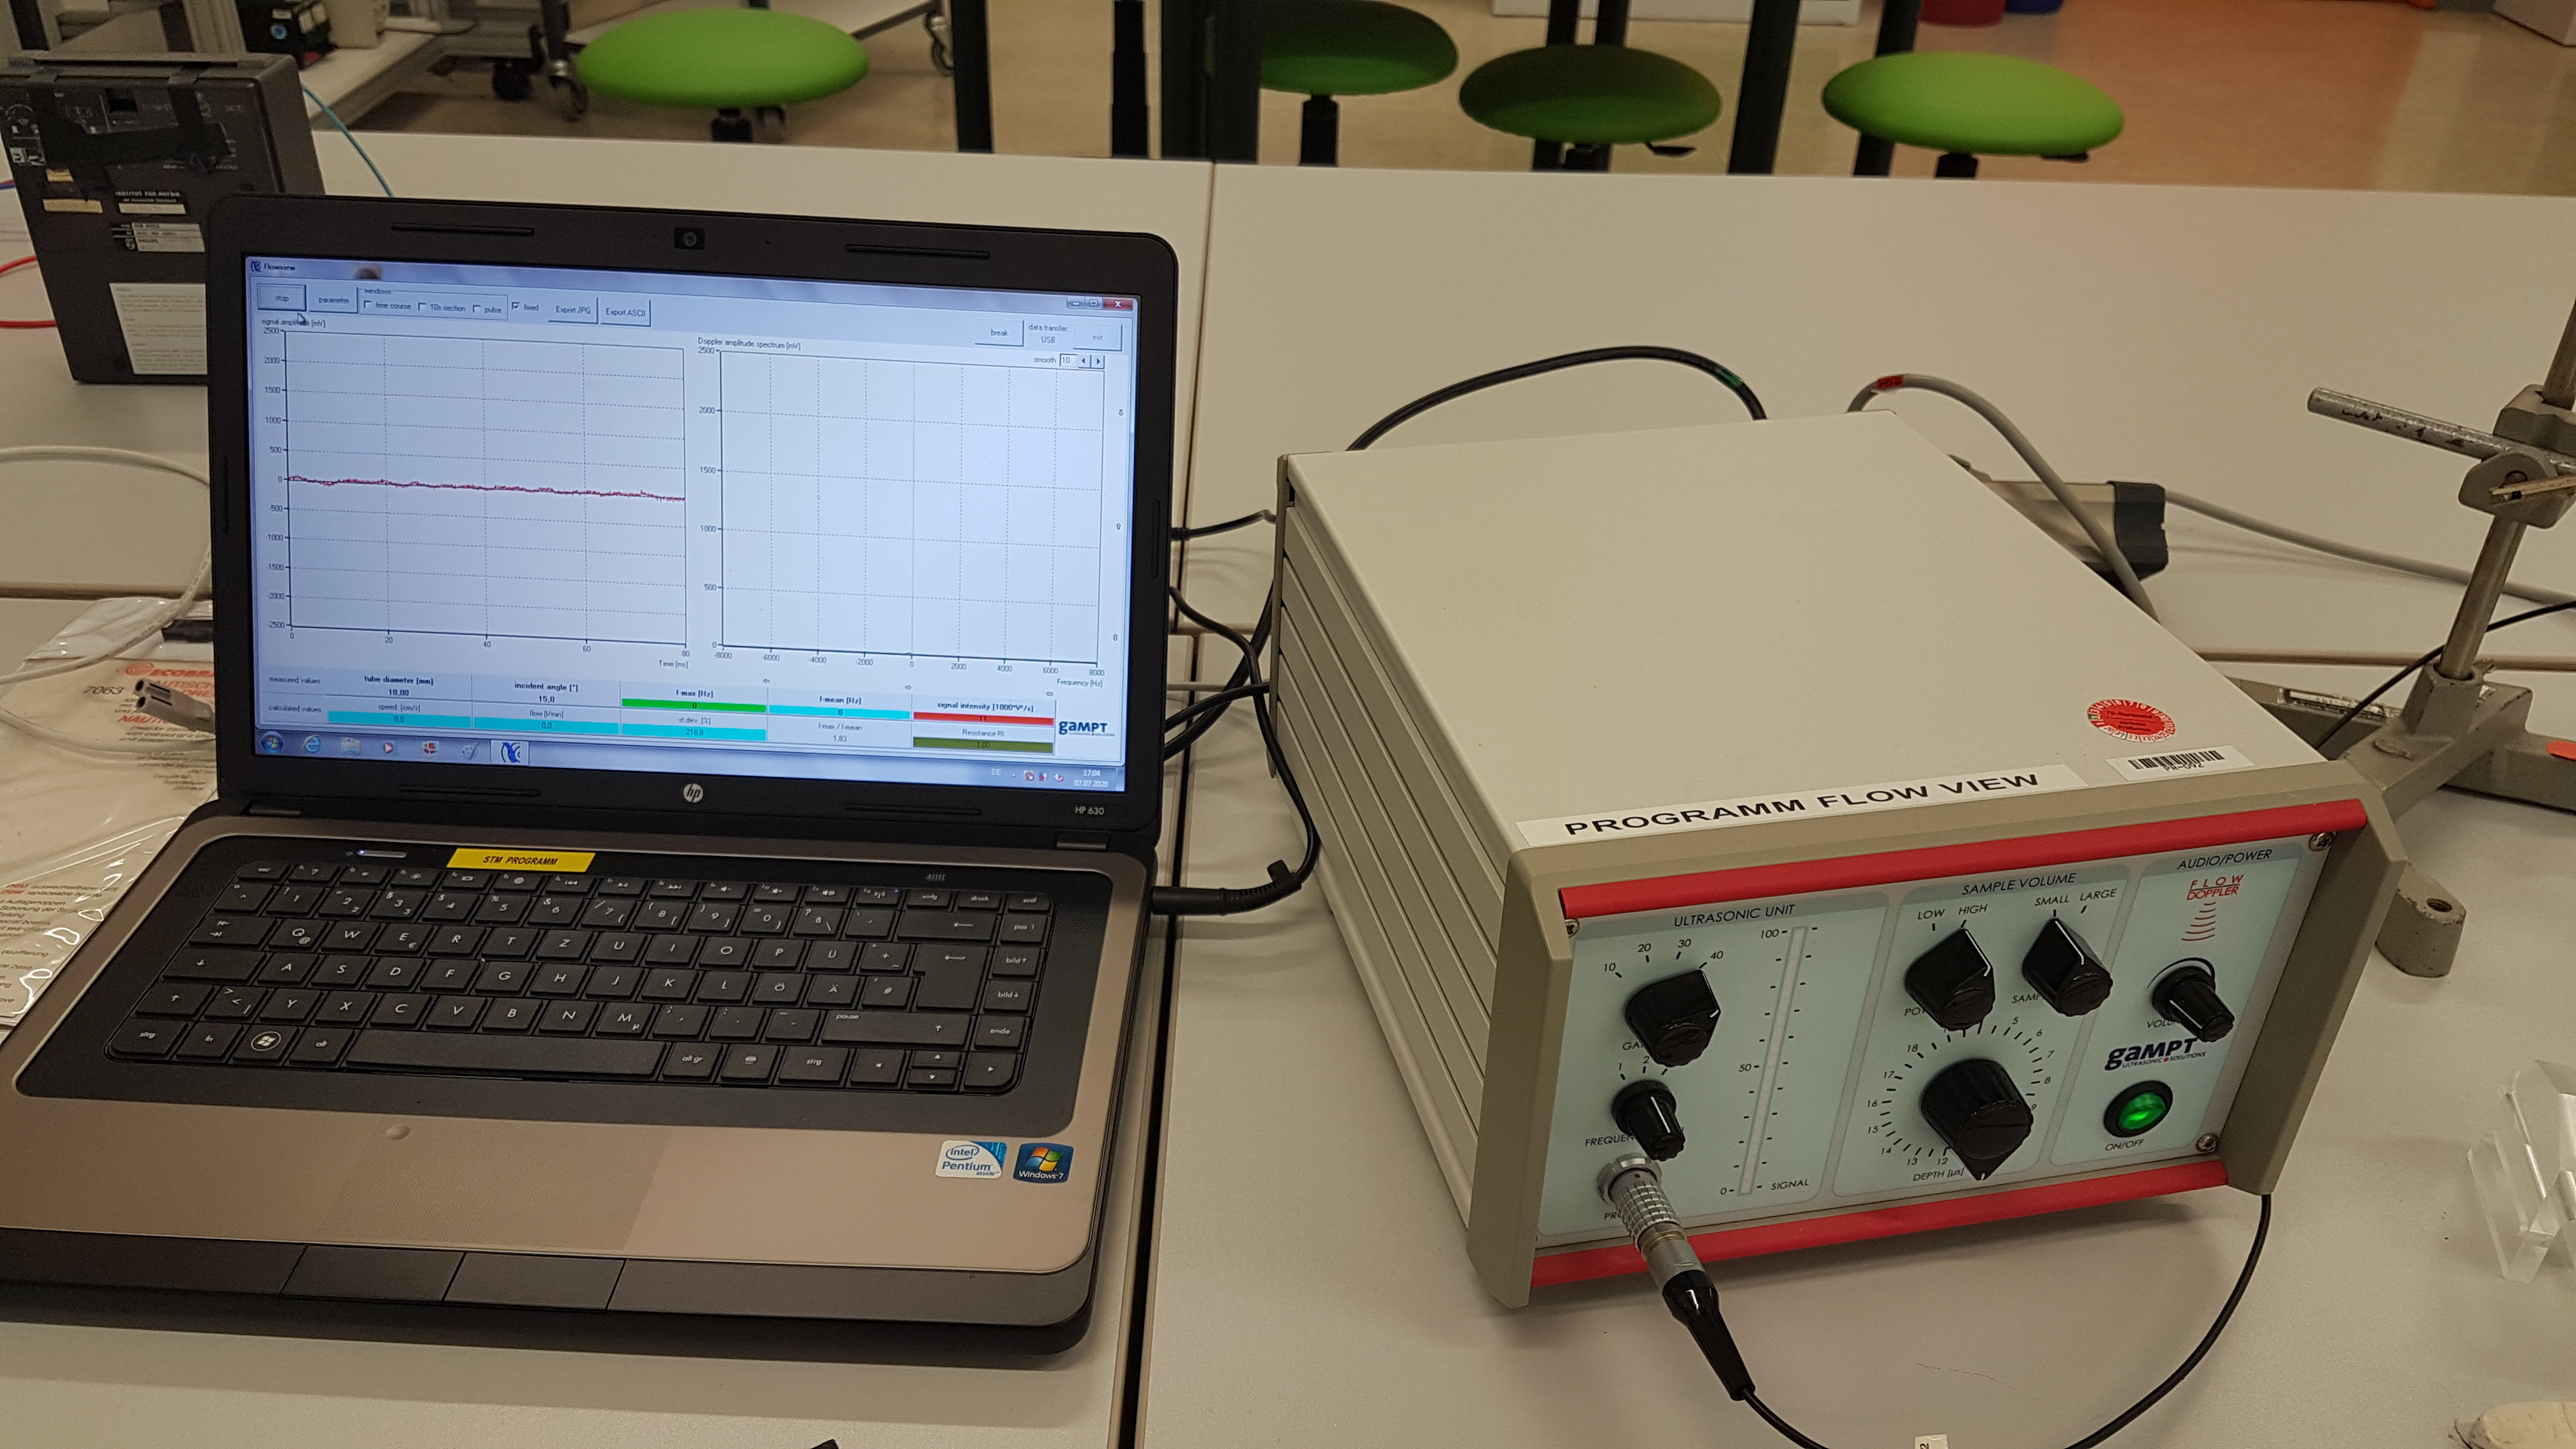
\includegraphics[width=0.75\linewidth]{images/Messaperatur.jpg}
    \caption{Hier ist die Messaperatur der Sonde abgebildet. Auf dem Laptop ist das UI des Programms FlowView zu erkennen, welches die Daten des rechts befindlichen Ultraschallgenerator 
    ausließt. Am Ultraschallgenerator kann zwischen den Einstellungen \textit{Small} und \textit{Large} unterschieden werden, welche für das Strömungsprofil und die Strömungsstärke relevant sind.
    Außerdem kann die Messtiefe unter der Einstellungen \textit{Small} variiert werden, was die Bestimmung des Strömungsprofils ermöglicht.}
    \label{fig:4}
\end{figure}

    \flushleft{Zu\;}\justifying Beginn wird der Ultraschallgenerator aus Abbildung \ref{fig:4} auf \textit{Large} gestellt um die Strömungsgeschwindigkeit bestimmen zu können. Anschließend wird zwischen
    dem Doppler-Prisma und dem Rohr Gel aufgetragen. Das gleiche wird für die Sonde an den drei Aufsetzpunkten wiederholt. Dann werden für die drei Winkel \SI{15}{\degree}, 
    \SI{30}{\degree} und \SI{45}{\degree} die Frequenzverschiebung $\Delta\nu$ dem Laptop entnommen. Dafür werden an der Pumpe nacheinander fünf Stärken eingestellt, für die jeweils ein Messwert 
    für die Frequenzverschiebung am Laptop abgelesen wird. Dies wird für jeden der drei Winkel wiederholt. Die fünf Stärken der Pumpe bleiben für alle drei Winkel gleich.\\
    Für das Strömungsprofil wird der Ultraschallgenerator auf \textit{Small} eingestellt. Es wird in dem Messintervall \SI{13.5}{\micro\second} bis \SI{19.5}{\micro\second} in \SI{0.5}{\micro\second} Schritten die 
    Frequenzverschiebung $\Delta\nu$ und die dazugehörige Signalstärke gemessen. 

\newpage
\section{Auswertung}

    \flushleft{Alle\;}\justifying folgenden Graphen werden mit der Python Bibliothek matplotlib \cite{matplotlib} und dessen Ausgleichgeraden mit dem Befehl polyfit aus der numpy Bibliothek 
    \cite{numpy} erstellt. Alle Fehler werden mithilfe der python Bibliothek uncertainties \cite{uncertainties} berechnet.\\
    \flushleft{Um\;}\justifying auf die Strömungsgeschwindigkeit der Doppler-Flüssigkeit zu schließen wird die Formel der Frequenzverschiebung $\Delta\nu$ \eqref{eq:3} zur Geschwindigkeit
    $v$ umgestellt, wodurch sich für die Geschwindigkeit folgendes Verhältnis ergibt:
    \begin{align}
        v &= \frac{1}{2} \frac{\Delta\nu \cdot c_L}{\nu_0\cdot \cos(\alpha)} \label{eq:5}
    \end{align}
    \flushleft{Als\;}\justifying Schallgeschwindigkeit wird hier die Schallgeschwindigkeit innerhalb der Doppler-Flüssigkeit
    $c_L=\text{\SI{1800}{\meter\per\second}}$ \cite{V903} verwendet. 

\newpage   
\subsection{Strömungsgeschwindigkeit für 15°}\label{sec:1}

    \flushleft{Aus\;}\justifying Formel \eqref{eq:5} lassen sich die Strömungsgeschwindigkeiten für die einzelnen Geschwindigkeiten der Pumpe bestimmen, welche in der Tabelle \ref{tab:5}
    zufinden sind. Mit den Werten aus Tabelle \ref{tab:1} für die Frequenzverschiebung $\Delta\nu$ und den daraus mit Formel \eqref{eq:5} berechneten Geschwindigkeiten aus Tabelle \ref{tab:5}, 
    lässt sich folgender Graph erstellen. Hier wird das Verhältnis $\sfrac{\Delta\nu}{\cos(\alpha)}$ gegen die jeweilige Strömungsgeschwindigkeit $v$ graphisch dargestellt, wobei der 
    Dopplerwinkel $\alpha$ mit Formel \eqref{eq:4} unter Verwendung des Winkels $\theta=15°$ bestimmt wird. 

\begin{figure}[H]
    \centering
    \includegraphics[width=0.75\linewidth]{build/plot15.pdf}
    \caption{Dieser Graph stellt die Strömungsgeschwindigkeit $v$ der Doppler-Flüssigkeit gegen das Verhältnis der Frequenzverschiebung $\Delta\nu$ mit dem Dopplerwinkel $\alpha$. 
    Der hier verwendete Winkel $\theta$ ist 15°. Die Ausgleichsgerade gibt einen strickt linearen Verlauf der berechneten Werte wieder.}
    \label{fig:5}
\end{figure}

    \flushleft{Für\;}\justifying diese und alle folgenden Ausgleichgeraden wird die Geradengleichung 
    \begin{align}
        v &= m \frac{\Delta\nu}{\cos(\alpha)} + b \label{eq:6}
    \end{align}
    \flushleft{verwendet.\;}\justifying
    Die für diesen Graphen relevanten Parameter der Steigung $m$ und des Schnittpunkts mit der $v$-Achse $b$ lauten wie folgt:
    \begin{align}
        m_{15°} &= \text{\input{m15.tex}} \label{eq:7}\\
        b_{15°} &= \text{\input{b15.tex}} \label{eq:8}
    \end{align}

\newpage
\subsection{Strömungsgeschwindigkeit für 30°}

    \flushleft{Für\;}\justifying die Winkel $\theta=30°$ und $\theta=45°$ wird analog zum Abschnitt \ref{sec:1} verfahren. Aus Formel \eqref{eq:5} und den Werten aus Tabelle \ref{tab:2}
    werden die Strömungsgeschwindigkeiten $v$ für die einzelnen Stärken der Pumpe berechnet. Der Dopplerwinkel $\alpha$ wird mit Formel \eqref{eq:4} bestimmt und in Formel \eqref{eq:5}
    eingesetzt. Werden die berechneten Strömungsgeschwindigkeiten aus Tabelle \ref{tab:6} gegen das Verhältnis $\sfrac{\Delta\nu}{\cos(\alpha)}$ graphisch aufgetragen ergibt sich folgender Graph:

\begin{figure}[H]
    \centering
    \includegraphics[width=0.75\linewidth]{build/plot30.pdf}
    \caption{Dieser Graph stellt die Strömungsgeschwindigkeit $v$ der Doppler-Flüssigkeit gegen das Verhältnis der Frequenzverschiebung $\Delta\nu$ mit dem Dopplerwinkel $\alpha$. 
    Der hier verwendete Winkel $\theta$ ist 30°. Die Ausgleichsgerade gibt einen strickt linearen Verlauf der berechneten Werte wieder.}
    \label{fig:6}
\end{figure}

    \flushleft{Die\;}\justifying für diesen Graphen relevanten Parameter der Steigung $m$ und des Schnittpunkts mit der $v$-Achse $b$ lauten wie folgt:
    \begin{align}
        m_{30°} &= \text{\input{m30.tex}} \label{eq:9}\\
        b_{30°} &= \text{\input{b30.tex}} \label{eq:10}
    \end{align}

\newpage
\subsection{Strömungsgeschwindigkeit für 45°}

    \flushleft{Im\;}\justifying folgenden Graph werden analog zu den Winkeln $\theta=15°$ und $\theta=30°$ die mit Formel \eqref{eq:5} berechneten Werte der Strömungsgeschwindigkeit 
    aus Tabelle \ref{tab:7} gegen das Verhältnis $\sfrac{\Delta\nu}{\cos(\alpha)}$ geplottet:

\begin{figure}[H]
    \centering
    \includegraphics[width=0.75\linewidth]{build/plot45.pdf}
    \caption{Dieser Graph stellt die Strömungsgeschwindigkeit $v$ der Doppler-Flüssigkeit gegen das Verhältnis der Frequenzverschiebung $\Delta\nu$ mit dem Dopplerwinkel $\alpha$. 
    Der hier verwendete Winkel $\theta$ ist 45°. Die Ausgleichsgerade gibt einen strickt linearen Verlauf der berechneten Werte wieder.}
    \label{fig:7}
\end{figure}

    \flushleft{Die\;}\justifying für diesen Graphen relevanten Parameter der Steigung $m$ und des Schnittpunkts mit der $v$-Achse $b$ lauten wie folgt:
    \begin{align}
        m_{45°} &= \text{\input{m45.tex}} \label{eq:11}\\
        b_{45°} &= \text{\input{b45.tex}} \label{eq:12}
    \end{align}

\newpage
\subsection{Strömungsprofil des Rohrs}

    \flushleft{Für\;}\justifying das Strömungsprofil wird die Strömungsgeschwindigkeit gegen die Messtiefe graphisch aufgetragen. Mit den Messwerten der Frequenzverschiebung
    $\Delta\nu$ aus Tabelle \ref{tab:4} und der Formel \eqref{eq:5} werden die Strömungsgeschwindigkeiten $v$ aus Tabelle \ref{tab:8} berechnet. Der Winkel $\theta$ ist hier
    15°. Werden die Strömungsgeschwindigkeiten gegen die Messtiefe aufgetragen ergibt sich der folgende Graph:

\begin{figure}[H]
    \centering
    \includegraphics[width=0.75\textwidth]{build/plotdepth.pdf}
    \caption{Dieser Graph stellt die Strömungsgeschwindigkeit $v$ an verschiedenen Messtiefen $d$ des Rohrs dar. Die maximale Strömungsgeschwindigkeit ist in rot und dessen dazugehörige
    Messtiefe in blau eingezeichnet.}
    \label{fig:8}
\end{figure}

\newpage
    \flushleft{Neben\;}\justifying der Messtiefe wird außerdem die Streuintensität der Messaperatur bestimmt. Dazu wird die Strömungsgeschwindigkeit gegen die Signalstärke aufgetragen.
    Die Messwerte zur Signalstärke werden der Tabelle \ref{tab:4} und die errechneten Strömungsgeschwindigkeiten der Tabelle \ref{tab:8} entnommen. Der daraus enstehende Graph
    sieht aus wie folgt:

\begin{figure}[H]
    \centering
    \includegraphics[width=0.75\textwidth]{build/plotstrength.pdf}
    \caption{Dieser Graph stellt die Strömungsgeschwindigkeiten $v$ gegen die Signalstärken der jeweiligen Frequenzverschiebung dar. Hier sind das Strömungsgeschwindigkeitsmaximum
    in rot und die maximale Signalstärke in blau eingezeichnet.}
    \label{fig:9}
\end{figure}

\newpage
\section{Diskussion}

    \flushleft{Die\;}\justifying Graphen \ref{fig:5}, \ref{fig:6} und \ref{fig:7} geben die Strömungsgeschwindigkeit in Anhängigkeit von der Frequenzverschiebung $\Delta\nu$ und
    dem Doppler-Winkel $\alpha$ an. Es ist ein deutliche lineares Verhältnis zwischen Geschwindigkeit und Frequenzverschiebung zu erkennen. Außerdem sind die Steigungen der 
    jeweiligen Ausgleichgeraden \eqref{eq:7}, \eqref{eq:9} und \eqref{eq:11} fast identisch. Dies lässt die Vermutung einer Unabhängigkeit des Beobachtungswinkels $\theta$ zu.\\
    Wird der Graph \ref{fig:8} betrachtet, lässt sich ein klares Maximum bei \SI{0.401}{\meter\per\second} erkennen. Daraus lässt sich schließen, dass die maximale Strömungsgeschwindigkeit
    bei einer Tiefe von \SI{17}{\micro\second} eintritt. Da die Tiefe von dem Doppler-Prisma (\SI{30.7}{\milli\meter} $\approx$ \SI{12}{\micro\second} \cite{V903}) von der gemessen Tiefe 
    abgezogen werden muss, ergibt sich eine tatsächliche Tiefe von \SI{5}{\micro\second}. Das entspricht einer Messtiefe von \SI{7.5}{\milli\meter}. Hierbei ist zu berücksichtigen,
    dass die Umrechnungsfaktoren für Acryl (dem Doppler-Prisma) und der Doppler-Flüssigkeit verschieden sind. Die Umrechnungsfaktoren lauten \SI{4}{\micro\second}=\SI{10}{\milli\meter}
    für Acryl und \SI{4}{\micro\second}=\SI{6}{\milli\meter} für die Doppler-Flüssigkeit \cite{V903}. Da die maximale Strömungsgeschwindigkeit im Zentrum des Rohres, also bei \SI{8}{\milli\meter}, 
    erwartet wird, ergibt sich der relative Fehler:
    \begin{align}
        \sigma_{\text{Tiefe}} &= \abs{\frac{7.5-8}{8}} = \text{\input{sigma.tex}} \label{eq:13}
    \end{align}
    \flushleft{Der\;}\justifying fehler ist relativ gering und könnte mit den empfindlichen Gerätschaften erklärt werden. Die Frequenzverschiebung, die über FlowView ausgelesen wurde, 
    schwankte stark, was eine genaue Bestimmung der Frequenzverschiebung für eine spezifische Pumpleistung erschwerte. Dies wird im folgenden Graphen nocheinmal verdeutlicht. Hier 
    werden die gemessenen Frequenzverschiebungen gegen die jeweiligen Pumpleistungen bei einem Winkel von $\theta=15°$ gegeneinander gestellt. 

\begin{figure}[H]
    \centering
    \includegraphics[width=0.75\textwidth]{build/plotdiskussion.pdf}
    \caption{Dieser Graph stellt die Frequenzverschiebung $\Delta\nu$ gegen die Pumpleistung bei einem Winkel $\theta=15°$ dar. Wird dieser Graph mit Graph \ref{fig:5} verglichen, fällt
    auf, dass der in Graph \ref{fig:5} inhomogene Abstand zwischen den einzelnen Messwerten mit einer zu niedrigen Frequenzverschiebung zu erklären ist.}
    \label{fig:10}
\end{figure}

    \flushleft{Der\;}\justifying vierte Messwert weicht ein wenig nach unten ab, was mit der starken Fluktuation der Frequenzverschiebung zusammenhängen könnte.\\
    Neben der schwankenden Frequenzverschiebung liefert der Graph \ref{fig:9} über die Signalstärke ein ähnliches Bild. Es ist auffällig, dass die Signalstärke ab den vierten
    Messwert anfängt zu streuen. Dennoch stimmt das Maximum der Signalstärke mit dem Maximum der Strömungsgeschwindigkeit aus Graph \ref{fig:8} überein. Ähnlich wie beim Ablesen
    der Frequenzverschiebung hat auch die Signalstärke stark geschwankt. Dies könnte auf die, zum Zentrum des Rohrs zunehmende, Strömungsgeschwindigkeit zurückführbar sein. 

\newpage
\printbibliography

\newpage
\section*{Appendix}
\addcontentsline{toc}{section}{Appendix}

\begin{table}[H]
    \centering
    \caption{In dieser Tabelle sind die Messwerte des Winkels $\theta=15°$ zu finden. Es wurde die Frequenzverschiebung $\Delta\nu$ für verschiedene Stärken der Pumpe gemessen.}
    \input{15.tex}
    \label{tab:1}
\end{table}

\begin{table}[H]
    \centering
    \caption{In dieser Tabelle sind die Messwerte des Winkels $\theta=30°$ zu finden. Es wurde die Frequenzverschiebung $\Delta\nu$ für verschiedene Stärken der Pumpe gemessen.}
    \input{30.tex}
    \label{tab:2}
\end{table}

\begin{table}[H]
    \centering
    \caption{In dieser Tabelle sind die Messwerte des Winkels $\theta=45°$ zu finden. Es wurde die Frequenzverschiebung $\Delta\nu$ für verschiedene Stärken der Pumpe gemessen.}
    \input{45.tex}
    \label{tab:3}
\end{table}

\begin{table}[H]
    \centering
    \caption{In dieser Tabelle sind die Messwerte der Frequenzverschiebung $\Delta\nu$, der jeweiligen Messtiefe $d$ und der Signalstärke zu finden. Diese wurden an dem großen
    Rohr mit einem Durchmesser von \SI{2.015}{\centi\meter} unter Verwendung des Winkels $\theta=15°$ gemessen.}
    \input{data.tex}
    \label{tab:4}
\end{table}

\begin{table}[H]
    \centering
    \caption{In dieser Tabelle sind die mit Formel \eqref{eq:5} berechneten Strömungsgeschwindigkeiten $v$ und die dazugehörigen Stärken der Pumpe bei einem Winkel von $\theta=15°$ 
    zu finden.}
    \input{v15.tex}
    \label{tab:5}
\end{table}

\begin{table}[H]
    \centering
    \caption{In dieser Tabelle sind die mit Formel \eqref{eq:5} berechneten Strömungsgeschwindigkeiten $v$ und die dazugehörigen Stärken der Pumpe bei einem Winkel von $\theta=30°$ 
    zu finden.}
    \input{v30.tex}
    \label{tab:6}
\end{table}

\begin{table}[H]
    \centering
    \caption{In dieser Tabelle sind die mit Formel \eqref{eq:5} berechneten Strömungsgeschwindigkeiten $v$ und die dazugehörigen Stärken der Pumpe bei einem Winkel von $\theta=45$ 
    zu finden.}
    \input{v45.tex}
    \label{tab:7}
\end{table}

\begin{table}[H]
    \centering
    \caption{In dieser Tabelle sind die mit Formel \eqref{eq:5} berechneten Strömungsgeschwindigkeiten $v$ und die dazugehörige Messtiefe $d$ und Signalstärke zu finden. Diese wurden
    unter Verwendung des Winkels $\theta=15°$ bestimmt und gemessen.}
    \input{v.tex}
    \label{tab:8}
\end{table}

\end{document}